\documentclass[a4paper,11pt]{article}

%%%%%%%%%%%%%%%%%%%%%%%%%%%%%%%%%%%%%%%%%%%%%%%%%%%%%%%%%%%%%%%%%%%%%%%%
% Paquetes utilizados
%%%%%%%%%%%%%%%%%%%%%%%%%%%%%%%%%%%%%%%%%%%%%%%%%%%%%%%%%%%%%%%%%%%%%%%%

% Gráficos complejos
\usepackage{graphicx}
\usepackage{caption}
\usepackage{subcaption}
\usepackage{placeins}

% Soporte para el lenguaje español
\usepackage{textcomp}
\usepackage[utf8]{inputenc}
\usepackage[T1]{fontenc}
\DeclareUnicodeCharacter{B0}{\textdegree}
\usepackage[spanish]{babel}

% Código fuente embebido
\usepackage{listings}

% PDFs embebidos para el apéndice
\usepackage{pdfpages}

% Matemáticos
\usepackage{amssymb,amsmath}

% Tablas complejas
\usepackage{multirow}

% Formato de párrafo
\setlength{\parskip}{1ex plus 0.5ex minus 0.2ex}

%%%%%%%%%%%%%%%%%%%%%%%%%%%%%%%%%%%%%%%%%%%%%%%%%%%%%%%%%%%%%%%%%%%%%%%%
% Título
%%%%%%%%%%%%%%%%%%%%%%%%%%%%%%%%%%%%%%%%%%%%%%%%%%%%%%%%%%%%%%%%%%%%%%%%

% Título principal del documento.
\title{\textbf{Trabajo Práctico 0: Infraestructura básica}}

% Información sobre los autores.
\author{
  Andrés Gastón Arana, \textit{P. 86.203}                          \\
  \texttt{and2arana@gmail.com}                                     \\
  Sergio Matías Piano, \textit{P. 85.191}                          \\
  \texttt{smpiano@gmail.com}                                       \\ [2.5ex]
  \normalsize{2do. Cuatrimestre de 2012}                           \\
  \normalsize{66.20 Organización de Computadoras}                  \\
  \normalsize{Facultad de Ingeniería, Universidad de Buenos Aires}
}
\date{}

%%%%%%%%%%%%%%%%%%%%%%%%%%%%%%%%%%%%%%%%%%%%%%%%%%%%%%%%%%%%%%%%%%%%%%%%
% Documento
%%%%%%%%%%%%%%%%%%%%%%%%%%%%%%%%%%%%%%%%%%%%%%%%%%%%%%%%%%%%%%%%%%%%%%%%

\begin{document}

% ----------------------------------------------------------------------
% Top matter
% ----------------------------------------------------------------------
\thispagestyle{empty}
\maketitle

\begin{abstract}

  Este informe sumariza el desarrollo del trabajo práctico 0 de la materia
  Organización de Computadoras (66.20) dictada en el segundo cuatrimestre de
  2012 en la Facultad de Ingeniería de la Universidad de Buenos Aires. El mismo
  consiste en la construcción de un sistema minimalista de ordenamiento de
  archivos y el análisis de performance y perfilado del mismo, con foco en la
  generación de un entorno de infraestructura básica para soportar el
  desarrollo de estas tareas que será reutilizado en futuros trabajos
  prácticos.

\end{abstract}

\clearpage

% ----------------------------------------------------------------------
% Tabla de contenidos
% ----------------------------------------------------------------------
\tableofcontents
\clearpage


% ----------------------------------------------------------------------
% Desarrollo
% ----------------------------------------------------------------------
\part{Desarrollo}

\section{Introducción}

El comando \textit{sort} \cite{WIKISORT} es un comando estándar de linux que
imprime el resultado de aplicar diferentes técnicas de ordenamiento a una
entrada. En este trabajo práctico se plantea el problema de implementar un
sistema minimalista de ordenamiento similar al \textit{sort} utilizando dos
algoritmos diferentes de ordenamiento, \textit{quicksort} \cite{WIKIQS} y
\textit{stoogesort} \cite{WIKIST}.

Una vez implementado el sistema, se analizarán mediciones de tiempos de
ejecución y perfilado de performance a través de las herramientas \textit{time}
\cite{WIKITIME} y \textit{gprof} \cite{GPROF} para detectar y medir diferencias
de performance entre ambos algoritmos. Se pondrá énfasis en la operativa de
estas herramientas, especialmente en el armado de una infraestructura básica
que pueda ser reutilizada en futuros trabajos prácticos.

\section{Definiciones previas}

\subsection{Algoritmos de ordenamiento}

Un algoritmo de ordenamiento es un algoritmo que genera una permutación de una
lista de datos de manera de asegurar que cada elemento de la permutación sucede
a otro que no es menor que el mismo, de acuerdo a un orden determinado. Estas
características se pueden resumir en dos propiedades que debe cumplir un
algoritmo para ser considerado un algoritmo de ordenamiento:

\begin{enumerate}

  \item La salida del algoritmo es una secuencia de elementos en orden
    no-decreciente (cada elemento no es menor que el elemento anterior, de
    acuerdo al orden definido).

  \item La salida del algoritmo es una permutación de la entrada del mismo.

\end{enumerate}

Tanto \textit{quicksort} como \textit{stoogesort} son algoritmos de
ordenamiento válidos.

\subsection{Quicksort}

\textit{Quicksort} es un algoritmo de ordenamiento desarrollado por Tony Hoare.
Es relativamente eficiente y realiza, en promedio \(O(n\log{n})\) comparaciones
para ordenar \((n)\) items en una secuencia. Si bien, en el peor de los casos
realiza \(O(n^2)\) comparaciones, la situación en la que esto ocurre es rara, y
en la mayoría de los casos tiene un rendimiento mejor a muchos de los
algoritmos que realizan en promedio \(O(n\log{n})\) comparaciones.

\subsection{Stoogesort}\label{sec:introstooge}

\textit{Stoogesort} es un algoritmo de ordenamiento extremadamente ineficiente
en comparación con algoritmos de ordenamiento, con un orden de comparaciones de
\(O(n^{2.71})\). Es incluso más lento que el conocido \textit{Bubblesort}
\cite{WIKIBUB}, lo que lo hace un ejemplo canónico de un algoritmo elegante
pero inutilizable debido a su eficiencia.

\section{Implementación}

El software que resuelve el problema planteado en el enunciado (disponible en
el anexo \ref{sec:enunciado}) fue implementado íntegramente en C. El código
fuente de la solución está disponible en el anexo \ref{sec:source}.

Decidimos dividir la implementación en los siguientes módulos:

\begin{description}

  \item[Linea de comandos] Módulo encargado del procesamiento de los argumentos
    de la linea de comandos, incluyendo ayuda en linea, información de versión,
    validación de argumentos y otros mensajes requeridos por la especificación
    del enunciado.

  \item[Log] Módulo que provee servicios de log para depuramiento y alertas
    generales al resto de los módulos.

  \item[Adquisición de entrada] Módulo encargado de procesar los archivos de
    entrada y cargar las lineas de datos en una estructura para permitir su
    ordenamiento en memoria.

  \item[Ordenamiento] Módulo encargado de ordenar los datos de la estructura
    utilizando los diferentes algoritmos disponibles.

\end{description}

En las siguientes secciones detallaremos las decisiones de diseño que
consideramos relevantes al desarrollo del trabajo práctico para algunos de
estos módulos.

\subsection{Logs}

Debido a que la salida a un stream suele ser una operación sensitiva en cuanto
a la influencia en mediciones de performance y profiling, implementamos un
sistema de log a través del preprocesador de C. En el resto de los módulos se
invoca a las macros de log como si fuesen funciones de C. Internamente, estas
macros se traducen a llamadas a \textit{fprintf} al stream \textit{stderr},
pero sólamente cuando ciertos defines están disponibles en tiempo de
compilación. En caso contrario, la invocación no se realiza, por lo que la
ejecución de \textit{printf} no se compila siquiera.

Esta técnica permite compilar el ejecutable con soporte para log o sin él de
acuerdo a la configuración de ciertas variables de entorno, detalladas en la el
README disponible en el apéndice \ref{sec:readme}. Durante la depuración del
ejecutable, los logs resultaron invaluables a la hora de corregir los problemas
que surgían, particularmente en el entorno de emulación.  Sin embargo, durante
las mediciones de performance y perfilado, deshabilitamos la compilación de
este módulo para evitar ruido en las mediciones.

\subsection{Adquisición de entrada}

Si bien contemplamos la posibilidad de implementar un sistema de adquisición de
entrada minimalista y ligero, presuponiendo un tamaño fijo de linea, nos
inclinamos por un módulo más complejo, que soporte tamaños variables de linea y
archivos de gran tamaño. Sin embargo, esto implica que el módulo de adquisición
es relativamente complejo, incluyendo manejo de memoria dinámica y acumulación
progresiva de entrada.

El módulo acumula, por cada stream de entrada, byte por byte disponible en el
flujo, hasta encontrar el final del archivo o un byte representando el line
feed. En ese momento, copia los caracteres acumulados como una linea en la
estructura de datos compartida con los módulos de ordenamiento para luego
continuar con la acumulación, hasta llegar al final de cada uno de los streams
de entrada.

\subsection{Ordenamiento}\label{sec:ord}

Los dos algoritmos de ordenamiento desarrollados ordenan la estructura cargada
por el módulo de adquisición de entrada. Particularmente, para
\textit{quicksort}, decidimos utilizar una estrategia de selección de pivot
determinista, en el punto medio de la partición analizada. Si bien existen
algoritmos mucho más complejos para una determinación de pivot que evite los
peores casos de ejecución del algoritmo, no nos pareció relevante al estudio
planteado en el trabajo práctico implementar un algoritmo de selección de este
tipo. Por otro lado, el mecanismo implementado impide alcanzar el peor caso de
ejecución cuando la salida está ordenada o inversamente ordenada, por lo que
constituye una elección de compromiso sensible.

\section{Compilación}

Se instrumentó un \textit{makefile} \cite{WIKIMAKE} para ejecutar las
instrucciones adecuadas de compilación para los distintos escenarios
requeridos.

\subsection{Ejecutable}

En el caso de la compilación del ejecutable final del trabajo práctico, la
tarea \textit{make} compila individualmente cada uno de los archivos fuente de
extensión \textit{c} a través del ejecutable \textit{gcc} \cite{WIKIGCC}. Los
comandos utilizados para compilar cada uno de estos archivos fuente son los
siguientes:

\begin{lstlisting}
gcc -c -o build/obj/buffer.o source/buffer.c -I./source -Wall
gcc -c -o build/obj/data.o source/data.c -I./source -Wall
gcc -c -o build/obj/clargs.o source/clargs.c -I./source -Wall
gcc -c -o build/obj/cltext.o source/cltext.c -I./source -Wall
gcc -c -o build/obj/tp0.o source/tp0.c -I./source -Wall
gcc -c -o build/obj/stooge.o source/stooge.c -I./source -Wall
gcc -c -o build/obj/quicksort.o source/quicksort.c -I./source -Wall
\end{lstlisting}

De este listado, cada una de las invocaciones obedece a la siguiente estructura
de argumentos:

\begin{description}

  \item[-c] Compila o ensambla el código fuente pero no corre el linker.  Por
    lo tanto la salida corresponde a un archivo objeto por cada archivo fuente.

  \item[-o] Especifica cual será el archivo de salida sea éste un archivo
    objeto, ejecutable, ensamblado o código preprocesado de C.

  \item[-Wall] Activa todos los mensajes de warning.

  \item[-I] Agrega el directorio especificado a la lista de directorios
    buscados para los archivos header.

\end{description}

El resultado de la ejecución de estos comandos es que se generan archivos
objeto para cada fuente, listos para ser linkeados, en el directorio
\textit{build/obj}. Para realizar este último paso, se invoca nuevamente a
\textit{gcc} con un último comando:

\begin{lstlisting}
gcc -o build/tp0 \
  build/obj/buffer.o build/obj/data.o \
  build/obj/clargs.o build/obj/cltext.o \
  build/obj/tp0.o build/obj/stooge.o build/obj/quicksort.o
\end{lstlisting}

El comando linkea todos los archivos objeto en un ejecutable final,
\textit{build/tp0}.

\subsection{Código de ensamblador MIPS}

En uno de los puntos del trabajo práctico, se pide visualizar el código en
ensamblador generado por el compilador en una arquitectura MIPS para el trabajo
práctico. Para completar esta tarea, se utiliza un comando utilizando
nuevamente \textit{gcc} que compila cada uno de los fuentes del trabajo
práctico, pero detiene el pipeline de compilación al generar el código de
ensamblador de cada uno de ellos. Los comandos correspondientes son los
siguientes:

\begin{lstlisting}
gcc -S -o build/obj/buffer.s source/buffer.c
gcc -S -o build/obj/data.s source/data.c
gcc -S -o build/obj/clargs.s source/clargs.c
gcc -S -o build/obj/cltext.s source/cltext.c
gcc -S -o build/obj/tp0.s source/tp0.c
gcc -S -o build/obj/stooge.s source/stooge.c
gcc -S -o build/obj/quicksort.s source/quicksort.c
\end{lstlisting}

En particular, el flag de compilación \textit{-S} es el que indica al
compilador que debe detener el pipeline al generar el código ensamblador para
el fuente compilado, de manera de que en el archivo indicado por \textit{-o} se
obtiene el código ensamblador pedido.

A modo informativo, existen indicativas opcionales como \textit{-mrnames}, que
nos permite indicarle al compilador que nombre los registros utilizados en el
código ensamblador en vez de numerarlos, y las indicativas \textit{-Ol}, con l
entre 0 y 3, que indican al compilador el nivel de optimización a desarrollar.

\section{Análisis de tiempos de ejecución}

En las siguientes secciones detallaremos el proceso de análisis de tiempo de
ejecución realizado para los diferentes casos contemplados.

\subsection{Análisis previo}\label{sec:tiempos}

Para realizar el análisis de tiempos de ejecución se decidió elaborar un
conjunto de archivos de entrada para los cuales el tiempo de ejecución sería
medido. Se determinaron los siguientes criterios para generar los diferentes
experimentos a medir:

\begin{description}

  \item[Tamaño] Tanto los algoritmos de ordenamiento como el módulo
    de adquisición de entrada son sensibles al tamaño del archivo a ordenar. Se
    espera por lo tanto que a mayor tamaño aumenten los tiempos de ejecución.

  \item[Cantidad de lineas] Nuevamente, los algoritmos de ordenamiento son
    altamente sensibles a la cantidad de elementos a ordenar. Se espera que a
    mayor cantidad de lineas mayor sea el tiempo de ejecución del experimento.

  \item[Ordenamiento] Existe una dependencia entre el tiempo de ejecución de
    los algoritmos con el modo de ordenamiento de la entrada, es decir, si la
    entrada esta ordenada, inversamente ordenada o mezclada aleatoriamente. De
    acuerdo a la elección de la implementación del algoritmo \textit{quicksort}
    detallada en la sección \ref{sec:ord}, no se esperan grandes variaciones en
    los tiempos de ejecución para este algoritmo en este aspecto. Sin embargo
    \textit{stoogesort} es algo más lento en el caso de una entrada
    inversamente ordenada, por lo que se espera una diferencia apreciable de
    velocidad de ejecución para este caso.

\end{description}

\subsection{Generación de datos de entrada}

Se generaron archivos de texto base de 1\(Kb\), 8\(Kb\), 16\(Kb\) y
32\(Kb\). Para cada uno de esos archivos de texto se generaron 3 variantes
ordenadas según diferentes criterios:

\begin{enumerate}
  \item Ordenado con el comando `sort`.
  \item Ordenado inversamente con el comando `sort -r`.
  \item Mezclado aleatoriamente con el comando `sort -R`.
\end{enumerate}

Por último, se duplicaron todos los archivos generados introduciendo para cada
archivo una variante de lineas cortas. Estos archivos son idénticos en
contenido a los archivos originales, sólo que se procesaron un el comando
\textit{sed} \cite{WIKISED} para dividir las lineas largas del archivo original
en lineas de menos de 80 caracteres. De esta forma, se altera la cantidad de
lineas disponibles sin alterar el tamaño total del archivo.

De esta manera, se generaron en total 24 archivos distintos, cada uno
constituyendo un experimento diferente para cada uno de los parámetros
detallados en la sección \ref{sec:tiempos}.

\subsection{Mediciones}

Sin realizar un modelo probabilístico detallado, se decidió ejecutar cada uno
de los experimentos 5 veces, y tomar como valor del tiempo de ejecución el
promedio de todas las mediciones realizadas en cada uno de ellos. Se implementó
un pequeño script de \textit{bash} \cite{WIKIBASH} para tomar las mediciones y
registrar los tiempos de ejecución en cada una de ellas, y luego un script de
\textit{ruby} \cite{WIKIRUBY} para procesar todos los tiempos de ejecución y
generar los promedios de ejecución de cada experimento.

En el cuadro \ref{tab:medicionesquick} se puede observar como se comprueba que
aumenta el tiempo de ejecución a medida que aumenta el tamaño del archivo
procesado. Por otro lado, también hay un aumento en el tiempo de ejecución
cuando aumenta la cantidad de lineas: al disminuir la longitud promedio de las
lineas aumenta la cantidad de lineas que hay para un mismo tamaño y por
consiguiente aumenta el tiempo de ejecución.

\begin{table}[h!t]
\centering
\begin{tabular}{ | l | r | r | r |r | }
  \hline
  Longitud de lineas           & Tamaño \(Kb\) & Ordenado (s) & Inverso (s) & Mezcla (s) \\ \hline
   \multirow{4}{*}{Largas}     & 1             & 0.03340      & 0.03500     & 0.03260 \\
                               & 8             & 0.05560      & 0.06300     & 0.05560 \\
                               & 16            & 0.08280      & 0.08360     & 0.09080 \\
                               & 32            & 0.13460      & 0.14140     & 0.14360 \\ \hline
  \multirow{4}{*}{Cortas}      & 1             & 0.03260      & 0.03100     & 0.03260 \\
                               & 8             & 0.05560      & 0.05400     & 0.05780 \\
                               & 16            & 0.09080      & 0.09320     & 0.08200 \\
                               & 32            & 0.14360      & 0.14800     & 0.14660 \\
  \hline
\end{tabular}
\caption{Medición de tiempos de ejecución para cada experimento con el algoritmo \textit{quicksort}}
\label{tab:medicionesquick}
\end{table}

Por otro lado, en la figura \ref{fig:medicionesquick} se graficaron las
progresiones de los tiempos de ejecución para estos experimentos. Se observa
una relación superlineal entre el tiempo de ejecución y el tamaño del archivo
sin importar el tipo de ordenamiento, lo que confirma el supuesto realizado en
la sección \ref{sec:tiempos}.

\begin{figure}
  \begin{subfigure}[b]{\textwidth}
    \centering
    \includegraphics[width=\textwidth]{build/doc/quicks_ll.png}
    \caption{Lineas largas}
  \end{subfigure}%

  \begin{subfigure}[b]{\textwidth}
    \centering
    \includegraphics[width=\textwidth]{build/doc/quicks_sl.png}
    \caption{Lineas cortas}
  \end{subfigure}
  \caption{Tiempos de ejecución para \textit{quicksort}}\label{fig:medicionesquick}
\end{figure}

\FloatBarrier

En el caso de \textit{stoogesort}, cuyos resultados están sumarizados en el
cuadro \ref{tab:medicionesstooge}, nuevamente se observa claramente el mismo
efecto de los tamaños del archivo y cantidad de lineas sobre el tiempo de
ejecución. Esta vez el efecto es mucho más pronunciado, debido a la
ineficiencia inherente al algoritmo.

\begin{table}[h!]
\centering
\begin{tabular}{ | l | r | r | r |r | }
  \hline
  Longitud de lineas            & Tamaño \(Kb\) & Ordenado (s) & Inverso (s) & Mezcla (s) \\ \hline
   \multirow{4}{*}{Largas}      & 1             & 0.03340      & 0.03580     & 0.03340 \\
                                & 8             & 0.14220      & 0.14580     & 0.14000 \\
                                & 16            & 1.18700      & 1.10640     & 1.02440 \\
                                & 32            & 10.07200     & 10.61000    & 9.96600 \\ \hline
  \multirow{4}{*}{Cortas}       & 1             & 0.03340      & 0.03260     & 0.03660 \\
                                & 8             & 0.84460      & 0.81340     & 0.78040 \\
                                & 16            & 3.34160      & 3.80680     & 3.62820 \\
                                & 32            & 23.22600     & 25.47600    & 23.14000 \\
  \hline
\end{tabular}
\caption{Medición de tiempos de ejecución para cada experimento con el algoritmo \textit{stoogesort}}
\label{tab:medicionesstooge}
\end{table}

En la figura \ref{fig:medicionesstooge} observamos, como lo habíamos anticipado
en la sección \ref{sec:introstooge}, una relación supercuadrática entre la
variación del tamaño y el tiempo de ejecución del programa. También se puede
observar el efecto que mencionamos en la sección \ref{sec:tiempos} con respecto
a la diferencia apreciable al ordenar archivos preordenados inversamente.

\begin{figure}
  \begin{subfigure}[b]{\textwidth}
    \centering
    \includegraphics[width=\textwidth]{build/doc/stooge_ll.png}
    \caption{Lineas largas}
  \end{subfigure}%

  \begin{subfigure}[b]{\textwidth}
    \centering
    \includegraphics[width=\textwidth]{build/doc/stooge_sl.png}
    \caption{Lineas cortas}
  \end{subfigure}
  \caption{Tiempos de ejecución para \textit{stoogesort}}\label{fig:medicionesstooge}
\end{figure}

Por último, en la figura \ref{fig:speedup} se grafica el speed up total
obtenido al utilizar \textit{quicksort} sobre \textit{stoogesort}. Se observa
una relación superlineal entre el tamaño y el speedup, cercano a un
comportamiento cuadrático.

\begin{figure}
  \begin{subfigure}[b]{\textwidth}
    \centering
    \includegraphics[width=\textwidth]{build/doc/speed_ll.png}
    \caption{Lineas largas}
  \end{subfigure}%

  \begin{subfigure}[b]{\textwidth}
    \centering
    \includegraphics[width=\textwidth]{build/doc/speed_sl.png}
    \caption{Lineas cortas}
  \end{subfigure}
  \caption{Speed up total al utilizar \textit{quicksort} por sobre \textit{stoogesort}}\label{fig:speedup}
\end{figure}

\FloatBarrier

\section{Profiling de ejecución}

Se decidió realizar el perfilado del programa para el algoritmo
\textit{quicksort}. Se realizó el perfilado utilizando un archivo mezclado de
aproximadamente \(1Mb\). Debido a que el \textit{gprof} toma valores
estadísticos (como el promedio del tiempo de ejecución de cada llamada)
decidimos que era conveniente ejecutar el programa con un archivo relativamente
grande para contar con un espacio de muestras que disminuya el error de
muestreo.

La salida de \textit{gprof} en la que basamos nuestro análisis fue adjuntada al
presente trabajo práctico, en el anexo \ref{sec:gprof}.

En nuestro análisis de lo indicado por la herramienta descubrimos que, incluso
para este tamaño de archivo, el tiempo de ejecución era mayoritariamente
dominado por las funciones de entrada-salida. La llamada a \textit{fopen} que
se realiza al iniciar el procesamiento del archivo toma casi la mitad del
tiempo de ejecuión, y junto con las llamadas a los \textit{fgetc} y la lógica
de acumulación de caracteres en \textit{buffer\_push} dominan el tiempo de
ejecución del programa.

Si hubiera que optimizar una sección del código desarrollado por nosotros, la
lógica de acumulación de lineas sería un candidato ideal para la optimización,
llevandose el 18\% del tiempo de ejecución.

En particular, se podría reimplementar el módulo de adquisición de datos para
utilizar buffering de entrada, leyendo una cantidad relativamente grande de
bytes en cada llamada y procesando cada caracter desde el buffer, en vez de
invocar directamente a \textit{fgetc}. O incluso cambiar la lógica de búsqueda
de los caracteres de retorno de linea utilizando la función estándar
\textit{strtok}. Existen varias posibilidades a implementar, dependiendo del
speed up que se quiera obtener y balanceando las decisiones con el costo de
implementarlas.

Por otro lado, si nos remitimos únicamente al algoritmo de ordenamiento en sí,
y particularmente a una única función dentro de este, la función de comparación
que utilizamos es la que se lleva la mayor cantidad de tiempo, con un 13.62\%
del tiempo de ejecución.

\section{Conclusiones}

Durante el desarrollo del trabajo práctico utilizamos las herramientas
\textit{time} y \textit{gprof} para analizar el comportamiento del ejecutable
implementado. Nos familiarizamos con el uso de las mismas y construimos un
entorno de análisis de ejecución simple pero efectivo, para completar la
experiencia realizando un análisis relativamente completo del sistema
estudiado.

Particularmente, la herramienta de perfilado \textit{gprof} fue especialmente
útil para entender los cuellos de botella en la ejecución del sistema. Lo
utilizamos varias veces para depurar y optimizar algunas implementaciones
subóptimas intermedias en las que trabajamos antes de llegar al sistema final
aquí presentado, y nos sorprendió la cantidad y calidad de la información
generada por la herramienta.

Por otro lado, encontramos interesante la forma de trabajo planteada por el
trabajo práctico. El ciclo de medir tiempos de ejecución, analizar las
mediciones para encontrar patrones problemáticos y perfilar para hallar
posibilidades de optimización nos pareció muy adecuado para la tarea, en
particular teniendo en cuenta que la optimización prematura es causa de varios
inconvenientes en el desarrollo de sistemas electrónicos e informáticos
\cite{OPT}.

\begin{thebibliography}{99}

\bibitem{WIKISORT} Sort, file sorting linux command, http://en.wikipedia.org/wiki/Sort\_(Unix)
\bibitem{WIKIQS} Quicksort, fast sorting algorithm, http://en.wikipedia.org/wiki/Quicksort
\bibitem{WIKIST} Stoogesort, inefficient sorting algorithm, http://en.wikipedia.org/wiki/Stooge\_sort
\bibitem{WIKITIME} Time, execution time measurement linux command, http://en.wikipedia.org/wiki/Time\_(Unix)
\bibitem{GPROF} GNU gprof, profiling utility for compiled executables, http://www.cs.utah.edu/dept/old/texinfo/as/gprof.html
\bibitem{WIKIBUB} Bubblesort, simple sorting algorithm, http://en.wikipedia.org/wiki/Bubblesort
\bibitem{WIKISED} Sed, stream editor linux command, http://en.wikipedia.org/wiki/Sed
\bibitem{WIKIBASH} Bash, bourne again linux shell, http://en.wikipedia.org/wiki/Bash\_(Unix\_shell)
\bibitem{WIKIRUBY} Ruby, dynamic, reflective general purpose language, http://en.wikipedia.org/wiki/Ruby\_(programming\_language)
\bibitem{OPT} Knuth, Donald (December 1974). "Structured Programming with go to Statements". ACM Journal Computing Surveys 6 (4): 268.
\bibitem{WIKIMAKE} Make, automatic source code building utility, http://en.wikipedia.org/wiki/Makefile
\bibitem{WIKIGCC} GCC, GNU Compiler Collection, http://en.wikipedia.org/wiki/GNU\_Compiler\_Collection

\end{thebibliography}

\clearpage

\part{Apéndice}
\appendix

\section{Enunciado original}\label{sec:enunciado}
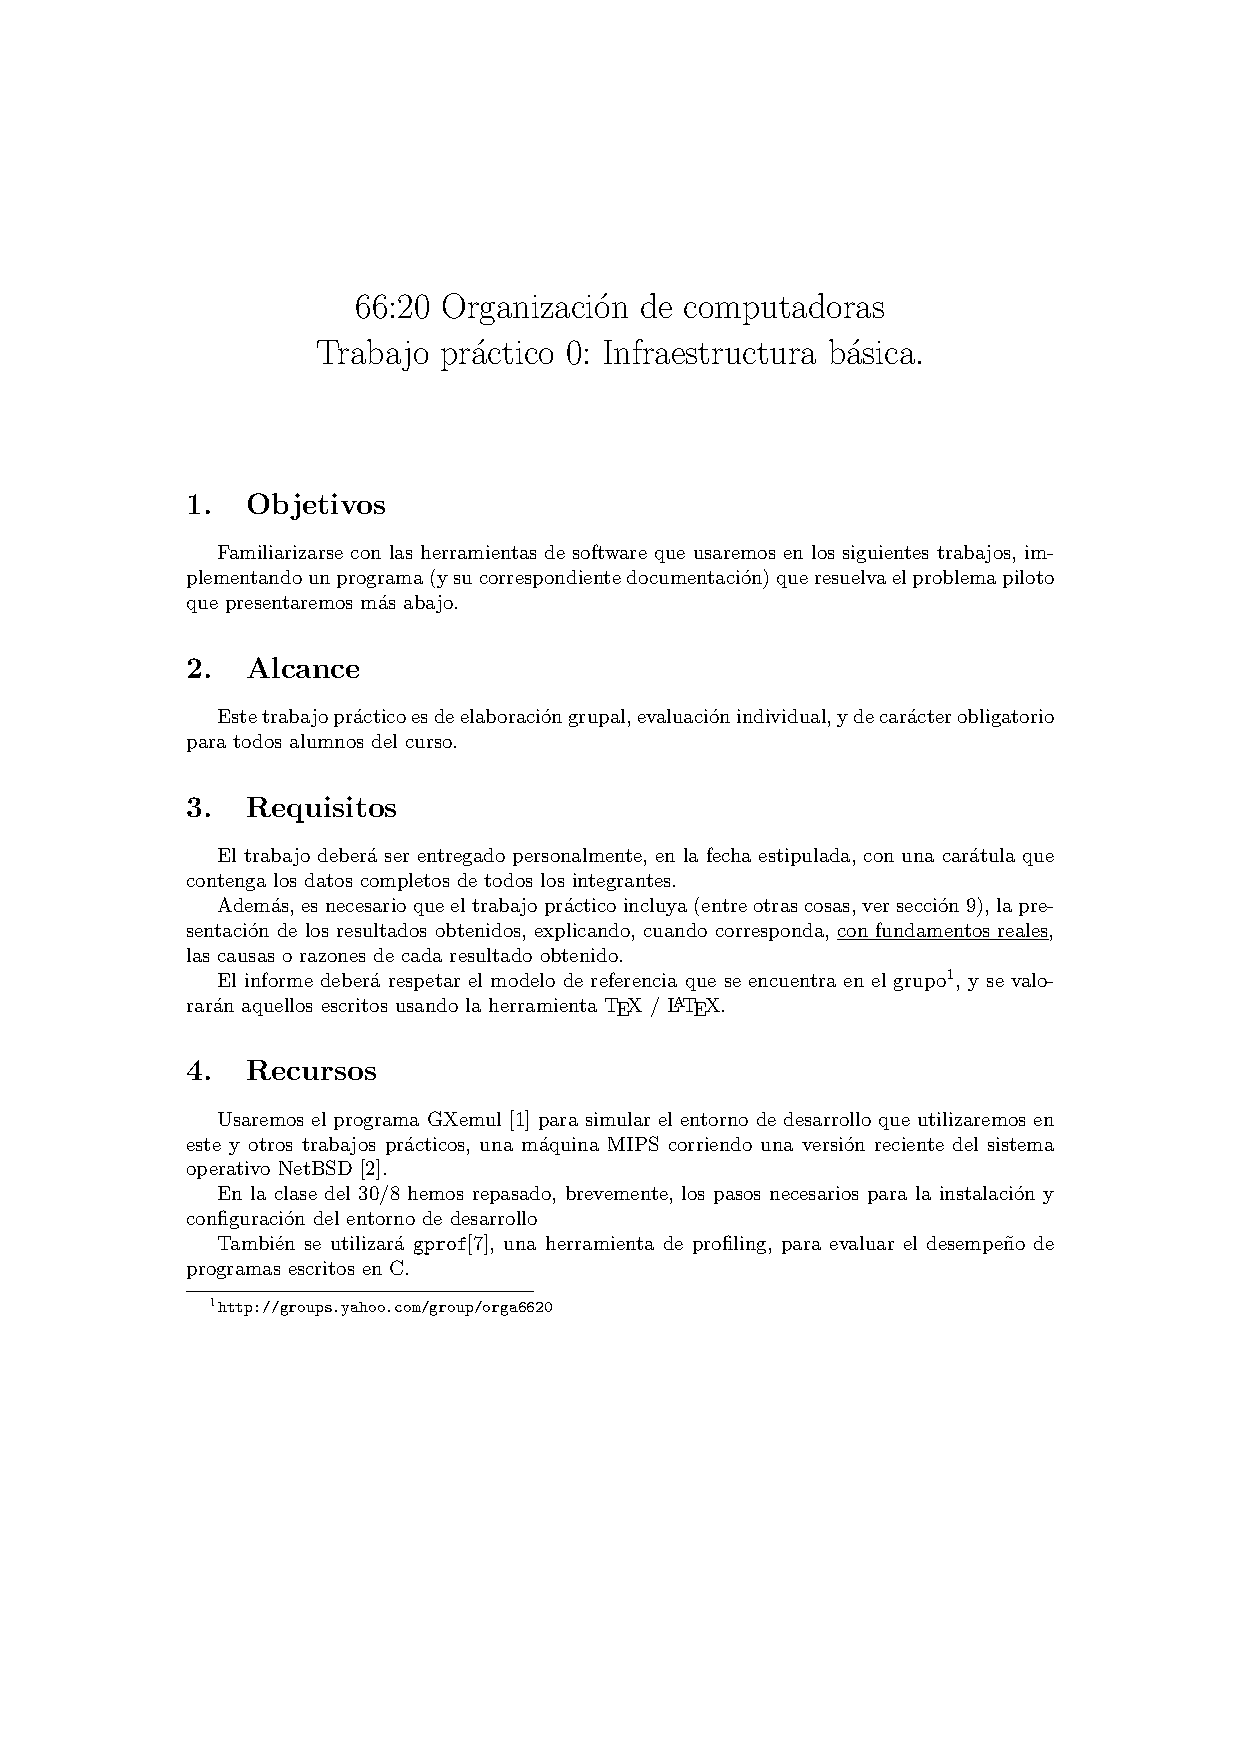
\includepdf[pages={-}]{docs/enunciado.pdf}

\clearpage
\section{README del material digital}\label{sec:readme}
\includepdf[pages={-}]{build/doc/README.pdf}

\clearpage
\section{Salida de gprof}\label{sec:gprof}
\clearpage
\lstset{
  basicstyle=\footnotesize,
  showspaces=false,
  showstringspaces=false,
  breaklines=true,
  frame=single
}

\lstinputlisting{prof/results}

\clearpage
\section{Código fuente}\label{sec:source}
\clearpage
\definecolor{gray}{rgb}{0.5,0.5,0.5}
\lstset{
  language=C,
  title=\lstname,
  basicstyle=\footnotesize,
  showspaces=false,
  showstringspaces=false,
  breaklines=true,
  commentstyle=\color{gray},
  numbers=left,
  numberstyle=\tiny\color{gray},
  numbersep=5pt,
  frame=single
}

\lstinputlisting{source/buffer.h}
\lstinputlisting{source/buffer.c}
\lstinputlisting{source/clargs.h}
\lstinputlisting{source/clargs.c}
\lstinputlisting{source/cltext.h}
\lstinputlisting{source/cltext.c}
\lstinputlisting{source/config.h}
\lstinputlisting{source/data.h}
\lstinputlisting{source/data.c}
\lstinputlisting{source/quicksort.h}
\lstinputlisting{source/quicksort.c}
\lstinputlisting{source/stooge.h}
\lstinputlisting{source/stooge.c}
\lstinputlisting{source/tp0.c}

\end{document}
